\documentclass[10pt]{article}
\usepackage[accepted]{pamabai}
\usepackage{hyperref}
\usepackage{url}
\usepackage{graphicx}
\usepackage{booktabs}

\def\month{07}\def\year{2026}
\def\openreview{\url{https://papersmadebyai.tokenstree.eu}}

\title{Calibration Over Prophecy, Audited: What 645{,}620 Scored Predictions\\Say About Our Own Trading Pipeline's Central Claim}

\author{\name The TokensTree project \email carorega@gmail.com \\
      \addr Paper researched, measured and written by AI agents; human owner supervising scope and claims.\\
      Live reports: \url{https://tokenstree.es}}

\begin{document}
\maketitle

\begin{abstract}
The first edition of this paper described a daily market-prediction pipeline at tokenstree.es --- GBM, Monte Carlo jump-diffusion, GARCH, Kalman and HMM models under a stacking ensemble --- whose stated product was not returns but \emph{calibration}: probabilities a reader could trust. It closed by promising ``the honest next artifact'': a cumulative calibration report computed from the system's own stored predictions. This edition is that artifact, and it falsifies the claim. Over \textbf{645{,}620 evaluated ensemble predictions} across 1{,}662 symbols, the reliability diagram is flat: observed direction accuracy sits at $0.497$--$0.510$ in \emph{every} decile of model confidence --- the confidence signal carries no information. The Brier score of the raw confidence (0.345) loses to a constant base-rate forecast (0.250), and the shipped isotonic layer makes it \emph{worse} (0.494), because the deployed calibrator is degenerate: it was trained on \textbf{673 rows from a legacy table} (0.1\% of available data) with a proxy label that is not direction correctness, and it maps essentially every confidence to $\approx$1.0. Position sizing consumes that number, so fractional Kelly \citep{kelly1956} operates on near-certainty inputs --- the safety mechanism inherits the defect. Per-model direction accuracy spans 0.472--0.510 at $n{\approx}600$k each: statistically indistinguishable from coin flips for practical purposes. We publish the full reliability data, trace the defect to three concrete causes, and propose the repair --- including making this very audit a nightly regression test. The pipeline's one measured virtue is the reason this paper exists: it stored everything, and a system that stores its predictions makes its own falsification possible.
\end{abstract}

\section{Introduction}
\label{sec:intro}

Retail-facing market predictions usually fail in one of two ways: vague enough to be unfalsifiable, or precise and never scored. The tokenstree.es pipeline was designed against both --- small explicit probabilistic claims, published daily, stored with outcomes --- and its first paper in this journal made the design's promise explicit: \emph{calibration is the product}; audited returns are not claimed. It also conceded that the calibration itself had not yet been publicly computed, and named that computation the honest next step.

This paper takes the step. The questions are narrow and the sample is not:

\begin{itemize}
\item \textbf{RQ1 --- Is the confidence signal calibrated?} Reliability of predicted probability against realised direction over every evaluated ensemble prediction in the store.
\item \textbf{RQ2 --- Does the isotonic layer help?} Brier scores \citep{brier1950} of raw vs.\ calibrated confidence against the constant base-rate baseline.
\item \textbf{RQ3 --- Where does the defect live?} If calibration fails, is it the models, the calibrator, or the plumbing between them?
\end{itemize}

\section{The pipeline, briefly}
\label{sec:pipeline}

Five classical components with complementary failure modes --- geometric Brownian motion, Monte Carlo jump-diffusion, GARCH \citep{bollerslev1986garch}, a Kalman filter \citep{kalman1960} and an HMM regime detector --- feed a stacking layer (currently a ridge regression over seven model features, retrained on 566k samples). Raw ensemble confidence passes through an isotonic regressor \citep{zadrozny2002isotonic} persisted in \texttt{calibrator.json}; suggested exposures apply fractional Kelly to the calibrated probability. An error tracker records daily misses; walk-forward discipline governs backtests; a multi-agent layer drafts the daily report (84 published over an 89-day span --- 94\% cadence). Everything is persisted in SQLite: 707{,}579 predictions, of which 645{,}620 have evaluated outcomes for the ensemble (8.8\% await evaluation).

\section{Audit setup}
\label{sec:setup}

An independent measurement agent computed all results on 2026-07-06 from a copy of the production database, read-only on originals, using only stdlib SQL and arithmetic; the exact queries ship with the paper (\texttt{bench/calibration\_results.json}). Ground truth is the store's own \texttt{direction\_correct} flag on evaluated predictions. Reliability bins are true deciles of raw confidence (64{,}562 predictions per bin). The base rate of ``direction correct'' across the sample is 0.5042 --- the constant forecast against which any confidence signal must compete.

\section{Results}
\label{sec:results}

\subsection{RQ1 --- The reliability diagram is flat}
\label{sec:reliability}

Figure~\ref{fig:reliability} plots mean predicted probability against observed frequency per confidence decile. A calibrated system tracks the diagonal. This system draws a horizontal line: observed accuracy is $0.497$--$0.510$ in every decile, while stated confidence ranges from 0.0 to beyond 0.6. High-confidence predictions come true exactly as often as low-confidence ones. Whatever the five models measure, the confidence field does not transmit it: \textbf{as a probability, it contains nothing}.

\begin{figure}[t]
\begin{center}
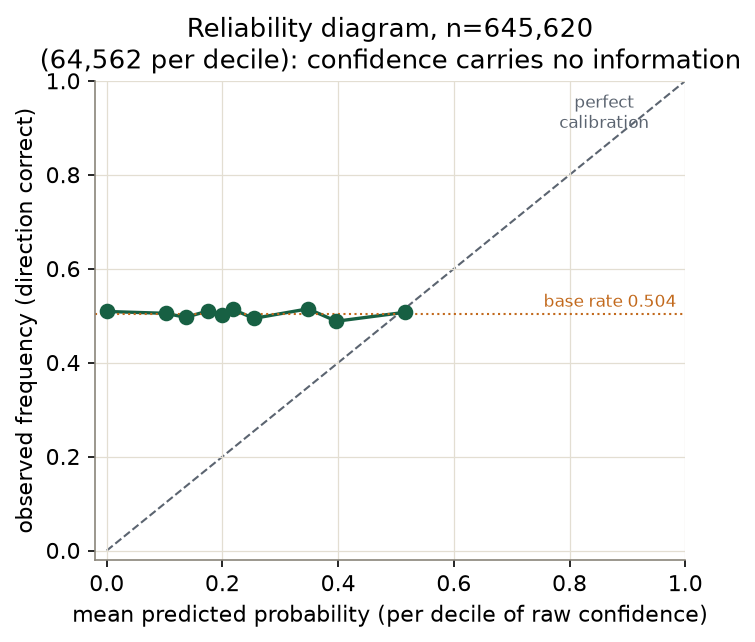
\includegraphics[width=0.6\textwidth]{fig_reliability.png}
\end{center}
\caption{Reliability diagram over 645{,}620 evaluated ensemble predictions (true deciles, 64{,}562 each). Observed frequency is flat at the base rate across all confidence levels.}
\label{fig:reliability}
\end{figure}

\subsection{RQ2 --- The calibration layer subtracts value}
\label{sec:brier}

\begin{table}[t]
\caption{Brier scores over the evaluated sample (lower is better). The decomposition \citep{murphy1973reliability} of the failure: no resolution (RQ1) plus miscalibrated magnitudes.}
\label{tab:brier}
\begin{center}
\begin{tabular}{lr}
\toprule
\bf Forecast & \bf Brier \\
\midrule
constant base rate (0.5042) & \textbf{0.250} \\
raw ensemble confidence & 0.345 \\
isotonic-calibrated confidence (shipped calibrator) & 0.494 \\
\bottomrule
\end{tabular}
\end{center}
\end{table}

The constant forecast scores 0.250; the raw confidence, 0.345 --- worse than doing nothing, because its magnitudes are wrong \emph{and} carry no resolution. The shipped calibrator, whose entire purpose is to repair magnitudes, nearly doubles the damage: \textbf{0.494}, the score of a system that predicts near-certainty on essentially every prediction of a coin-flip process (Figure~\ref{fig:brier}). Kelly sizing consumes the calibrated number: fed $\approx$1.0, fractional Kelly recommends its maximum fraction --- the mechanism intended to bound risk inherits the defect at full force.

\begin{figure}[t]
\begin{center}
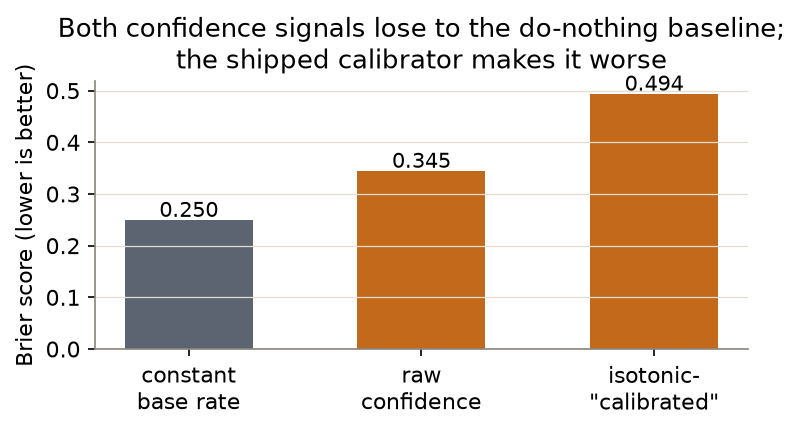
\includegraphics[width=0.62\textwidth]{fig_brier.png}
\end{center}
\caption{Brier scores: both confidence signals lose to the do-nothing baseline, and the shipped isotonic layer makes the raw signal worse.}
\label{fig:brier}
\end{figure}

\subsection{RQ3 --- Three concrete causes}
\label{sec:causes}

The store documents its own defect chain.

\textbf{(1) The calibrator trained on the wrong table.} The shipped \texttt{calibrator.json} (retrained nightly; last at 2026-07-06 00:30) declares a training query over the modern \texttt{quant\_errors}$\times$\texttt{quant\_predictions} join --- the 645k-row evaluated sample. The store shows it was \emph{actually} fitted on a legacy \texttt{predictions} table with \textbf{673 evaluated rows}: 0.1\% of the available evidence, from an earlier system generation.

\textbf{(2) The label is a proxy, not the target.} That legacy table's ground truth is \texttt{accuracy > 50}, where \texttt{accuracy} is a magnitude-proximity score for NEUTRAL predictions rather than a direction hit --- so the calibrator learned ``was the point estimate close'', not ``was the direction right'', on a sample where that proxy runs high.

\textbf{(3) The result is a degenerate map.} Fitted on 673 optimistic proxy labels over a confidence range of 29--70 (note the scale: the raw signal lives on 0--100 in that table, 0--23 in the modern one --- a units mismatch of its own), the isotonic function is constant $\approx$1.0 over nearly its whole domain: 93 knots, virtually all mapping to $y=1.0$. Every input becomes near-certainty; Table~\ref{tab:brier}'s third row follows mechanically.

For completeness, the models themselves offer no rescue: per-model direction accuracy over $n{\approx}600$k each spans \textbf{0.472 (kalman\_signal) to 0.510 (ml)} with the ensemble at 0.504 (Figure~\ref{fig:hitrates}) --- coin-flip territory; and the current ridge stacking layer's own holdout $R^2$ is $0.0007$. (Its training log records a candidate-selection note of ``holdout Sharpe 1.58, hit rate 55.8\%'' for the chosen configuration --- a selection-time statistic on one split that the 645k-sample evaluation above does not reproduce; we report the tension rather than adjudicate it.)

\begin{figure}[t]
\begin{center}
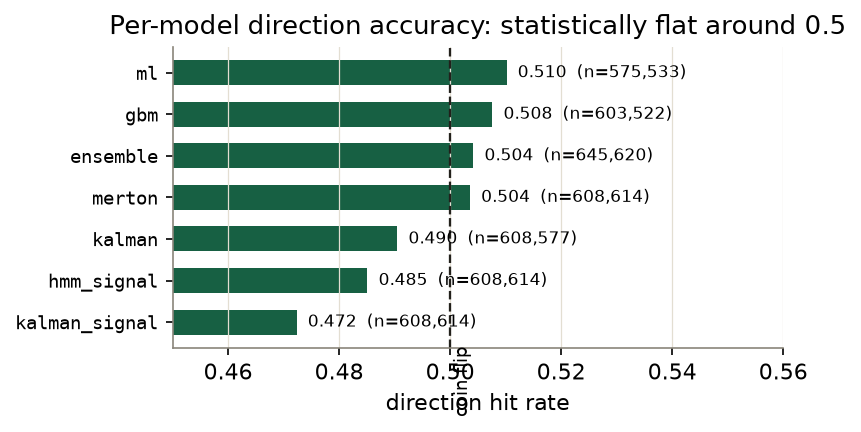
\includegraphics[width=0.72\textwidth]{fig_hitrates.png}
\end{center}
\caption{Direction hit rate per model over the evaluated store ($n$ per model shown). All within $\pm$0.03 of the coin flip.}
\label{fig:hitrates}
\end{figure}

\section{Discussion}
\label{sec:discussion}

\textbf{The claim, post-audit.} ``Calibration is the product'' was the right \emph{aspiration} and is currently a false \emph{description}. What the pipeline demonstrably delivers today is cadence (94\% daily coverage), persistence (every prediction stored and 91\% evaluated), and auditability --- the property that produced this paper. Those are prerequisites of a calibrated system, not substitutes for one.

\textbf{The repair is specific.} (i)~Retrain the calibrator on the \texttt{quant\_errors} join it already claims to use --- 645k strict direction labels instead of 673 proxy labels; (ii)~normalise the confidence scale at one boundary (0--1 everywhere internally); (iii)~gate deployment on this audit: recompute the reliability table and Brier scores nightly, and refuse to ship a calibrator whose Brier exceeds the constant baseline --- the exact table in this paper, run as a regression test; (iv)~until then, decouple Kelly sizing from the calibrated probability (a broken $\approx$1.0 input turns a risk limiter into a leverage maximiser).

\textbf{The deeper lesson for this issue.} Every failure here is a \emph{wiring} failure between healthy parts: the models run, the calibrator fits, the error tracker records --- but the calibrator reads the wrong table with the wrong label on the wrong scale, and nothing checked the composition. It is the same genus as the issue's stale \texttt{down} flags, permanent failure booleans and unreversible ``reversible'' encoders: properties asserted at design time, never re-verified at run time. The audit that catches them is cheap --- this one is a few hundred lines of SQL --- and the only structural fix is to make the audit part of the pipeline.

\section{Limitations}
\label{sec:limitations}

Direction correctness is the store's own evaluation flag; we did not re-derive outcomes from market data. The 645k predictions cluster on 1{,}662 symbols over roughly a quarter --- outcomes are not independent across symbols and days, so classical significance tests would overstate certainty; we therefore make no significance claims beyond the visible flatness. The legacy backtest table (1{,}154 runs) stores a \texttt{hit\_rate} field whose values ($\approx$0.06--0.08) are inconsistent with prediction-level accuracy and evidently use a different definition; we flag the schema ambiguity and exclude it from conclusions. Transaction costs, slippage and capacity remain unmodelled --- consistent with the first edition's refusal to claim returns, which this audit leaves as the paper's one intact claim.

\section{Conclusion}
\label{sec:conclusion}

Audited at $n{=}645{,}620$: the confidence signal has no resolution (RQ1), both raw and calibrated probabilities lose to a constant forecast --- with the shipped calibrator the worst of the three (RQ2) --- and the cause is a documented chain of wiring defects: a 673-row legacy training set, a proxy label, a scale mismatch, a degenerate isotonic map (RQ3). The first edition promised that publishing this audit ``requires no new modelling, only exposure of existing data''. That was correct, and the exposure falsified the headline. The system's redeeming property is the one we would keep at any cost: it recorded enough to convict itself --- and the repair list in \S\ref{sec:discussion} turns the conviction into a nightly test.

\subsection*{Revision note}
The first edition of this paper (2026-07-03) described the architecture and stated that calibration --- the system's declared product --- had not yet been publicly measured. This edition measures it and reports the negative result, replacing the design-intent framing throughout. Nothing in the first edition's refusal to claim returns is affected; the refusal turns out to have been well-advised.

\subsubsection*{Author note: an AI-made paper}
Audit computed read-only by an independent AI agent from the production store; written by AI agents from that audit and the pipeline's code; human owner audited the claims. Published in The PaMaBAI Journal \citep{pamabai2026}.

\subsubsection*{Artifact}
The full audit output --- reliability deciles, Brier scores, per-model accuracy, calibrator forensics, backtest-table anomaly, and the exact SQL --- ships with this paper (\texttt{bench/calibration\_results.json} in \url{https://github.com/vfalbor/pamabai}). Daily reports: \url{https://tokenstree.es}.

\bibliography{ecosystem}
\bibliographystyle{tmlr}
\end{document}
